\section{Introduction}
Remembering where a vehicle was parked has proven a hassle in large parking structures. Existing RF signature based indoor localization technology is not applicable where such signals may not be available such as at underground parking lots.
Instrumenting additional sensors may solve the problem but at the cost of significant overheads in time, money and human efforts. 

\iffalse
(Problem)
With the rapid growth of personal vehicles amount and growth of urban parking spaces demands, there appear numerous large parking facilities, most of which are built underground. Drivers may find it a nightmare to search for their vehicles in the dim and mazelike parking lot since the parking lots are very large and have similar appearance inside without visual features.

(Why it's hard to solve) Localizing a vehicle in a parking lot is a challenging problem due to the special environment most parking lots have. Although most vehicles are equipped with vehicle-mounted GPS and the mobile devices of the driver also have GPS, the indoor environment especially underground environment makes it impractical to use GPS. Radio Frequency (RF) fingerprinting of WiFi signals which has been a popular approach to indoor localization \cite{bahl00radar, youssef2005horus} do not work here since the poor WiFi coverage in the parking lots. An optional solution is to install additional infrastructure(e.g. sensor network), however, this method is effort-intensive and costly, also, this kind of installation may be infeasible in many parking lots already built.
\fi

%An ideal solution should work without the aid of such additional environmental sensors, and it should provide accurate enough location of the vehicle to the driver even where GPS and RF signals are weak or unavailable. Only then can it be applicable to general enough scenarios such as underground and legacy parking lots.


%(Ideal solution)
%Common used smartphone is an ideal choice to address this problem. Inertial sensors inside the smartphone can provide cues for localization vehicles. If the result of localization can be recorded on the smartphone, the driver could use his smartphone to find his car when he comes back. In addition, informing drivers the map of the parking lot and the real-time position of the vehicle would be helpful for drivers to search for an unoccupied parking place especially in an unfamiliar environment.

%(Effects)

%In this paper, we propose 
VeLoc is a vehicle localization system that utilizes accelerometer and gyroscope sensors in the smartphone to provide accurate vehicle localization. It does not rely on GPS or RF signals, neither require any additional sensors to instrument the parking ground. %Instead, the driver simply runs the VeLoc application before entering a parking structure. VeLoc will track the vehicle movements, estimate its location, and record where the vehicle is finally parked.% This information is then used to direct the driver back to the parked spot when she/he returns.

%The intuition behind VeLoc is that although a noisy trajectory does not, by itself, reveal a vehicle's location, using the constraints imposed by the parking structure��s map and detected landmarks is able to help vehicle tracking(shown in Figure \ref{fig_poster}).
%This is because (a) trajectories can be used for localization since only a few paths on the map could accommodate the trajectory. (b) once a landmark is detected, only a few positions marked with the same kind of landmark are possible. (c) using both map constraints and detected landmark could narrow down the uncertainty more quickly and trace a vehicle more accurately.
%This is because (i) there may be only a few paths on the map that could accommodate the trajectory as shown in Figure \ref{fig_apf_intuition1}.
%(ii) A detected landmark (e.g., a bump, turning or slope) can further pin down the positions where a vehicle might be (as shown in Figure \ref{fig_apf_intuition2}) since there are limited number of such landmarks on the map. Hence, using the synergy of both constraints is able to narrow down the uncertainty more quickly and trace a vehicle more accurately (as shown in Figure \ref{fig_apf_intuition3}).


%We design several algorithms and implement a real-time system to localize a vehicle using a smartphone inside with arbitrary pose and possible jolting. No installation of additional infrastructure is needed and all what users need to do during a drive is to run the VeLoc to process collected data. Finally, VeLoc provides localization result for usrs to find their car when they come back latter.

%(Difficulties)
Realizing such an inertial-based solution, however, involves non-trivial challenges. First, the driver may place the phone in arbitrary positions and road conditions may jolt the phone to change its position on the course. How to estimate the pose (i.e., the relative orientation of the smartphone to the vehicle) despite all such uncertainty and disturbances? Second, %although admirable work has been done~\cite{ParkSense,Lindqvist:Undistracted_Driving} to estimate the walking distance of a person,
inferring the vehicle's traveling distance or even trajectory is still difficult due to the lack of periodic acceleration patterns, which are fundamental in step-counting techniques~\cite{ParkSense,Lindqvist:Undistracted_Driving}. %Although landmarks of unique acceleration, magnetism patterns such as escalators can calibrate the location~\cite{Wang:UnLoc},
Also, identifying which types of landmarks can be reliably recognized despite different parking lots, vehicles and driving styles, and how, remain open questions. Finally, since both the pose and landmark detection results contain errors, how can one track the location of a vehicle accurately, such that the driver can always find the vehicle? % tracking the vehicle in real time requires efficient computation that can fit the resources available on smartphones.

%(High-level description)
%VeLoc contains several components to deal with the above challenges.
%A \textit{Pose estimation} algorithm estimates the pose of the smartphone inside the vehicle, regardless of how the phone is oriented relative to the vehicle and occasional changes in its pose due to bumpy driving. We also develop a \textit{Landmark detection} algorithm which uses pattern recognition and machine learning techniques~\cite{} to find unique patterns corresponding to different types of landmarks and implement real-time classification algorithm to detect them reliably.
%Finally, we represent the uncertainty about the state of the vehicle explicitly as probability distributions. We incorporate the uncertainty arising from sensing and the parking structure's map information provided by the map or detected landmarks, into a novel Bayes Filtering framework, specifically, \textit{ Augmented Particle Filtering} framework to simultaneously harness constraints imposed by the map and landmark detection for localization. (xx last sentence still too long and vague. need to sharpen the point)

%(High-level description)
As shown in Figure~\ref{pix:overview}, VeLoc contains three components to deal with the above challenges.
A \textit{pose estimation} module estimates the pose of the smartphone inside the vehicle. A \textit{landmark detection} module finds unique patterns corresponding to different types of landmarks and classify them reliably. A \textit{location estimation} module determines the vehicle's final location from the map and detected landmarks. 

\begin{figure}[h]
  \centering
  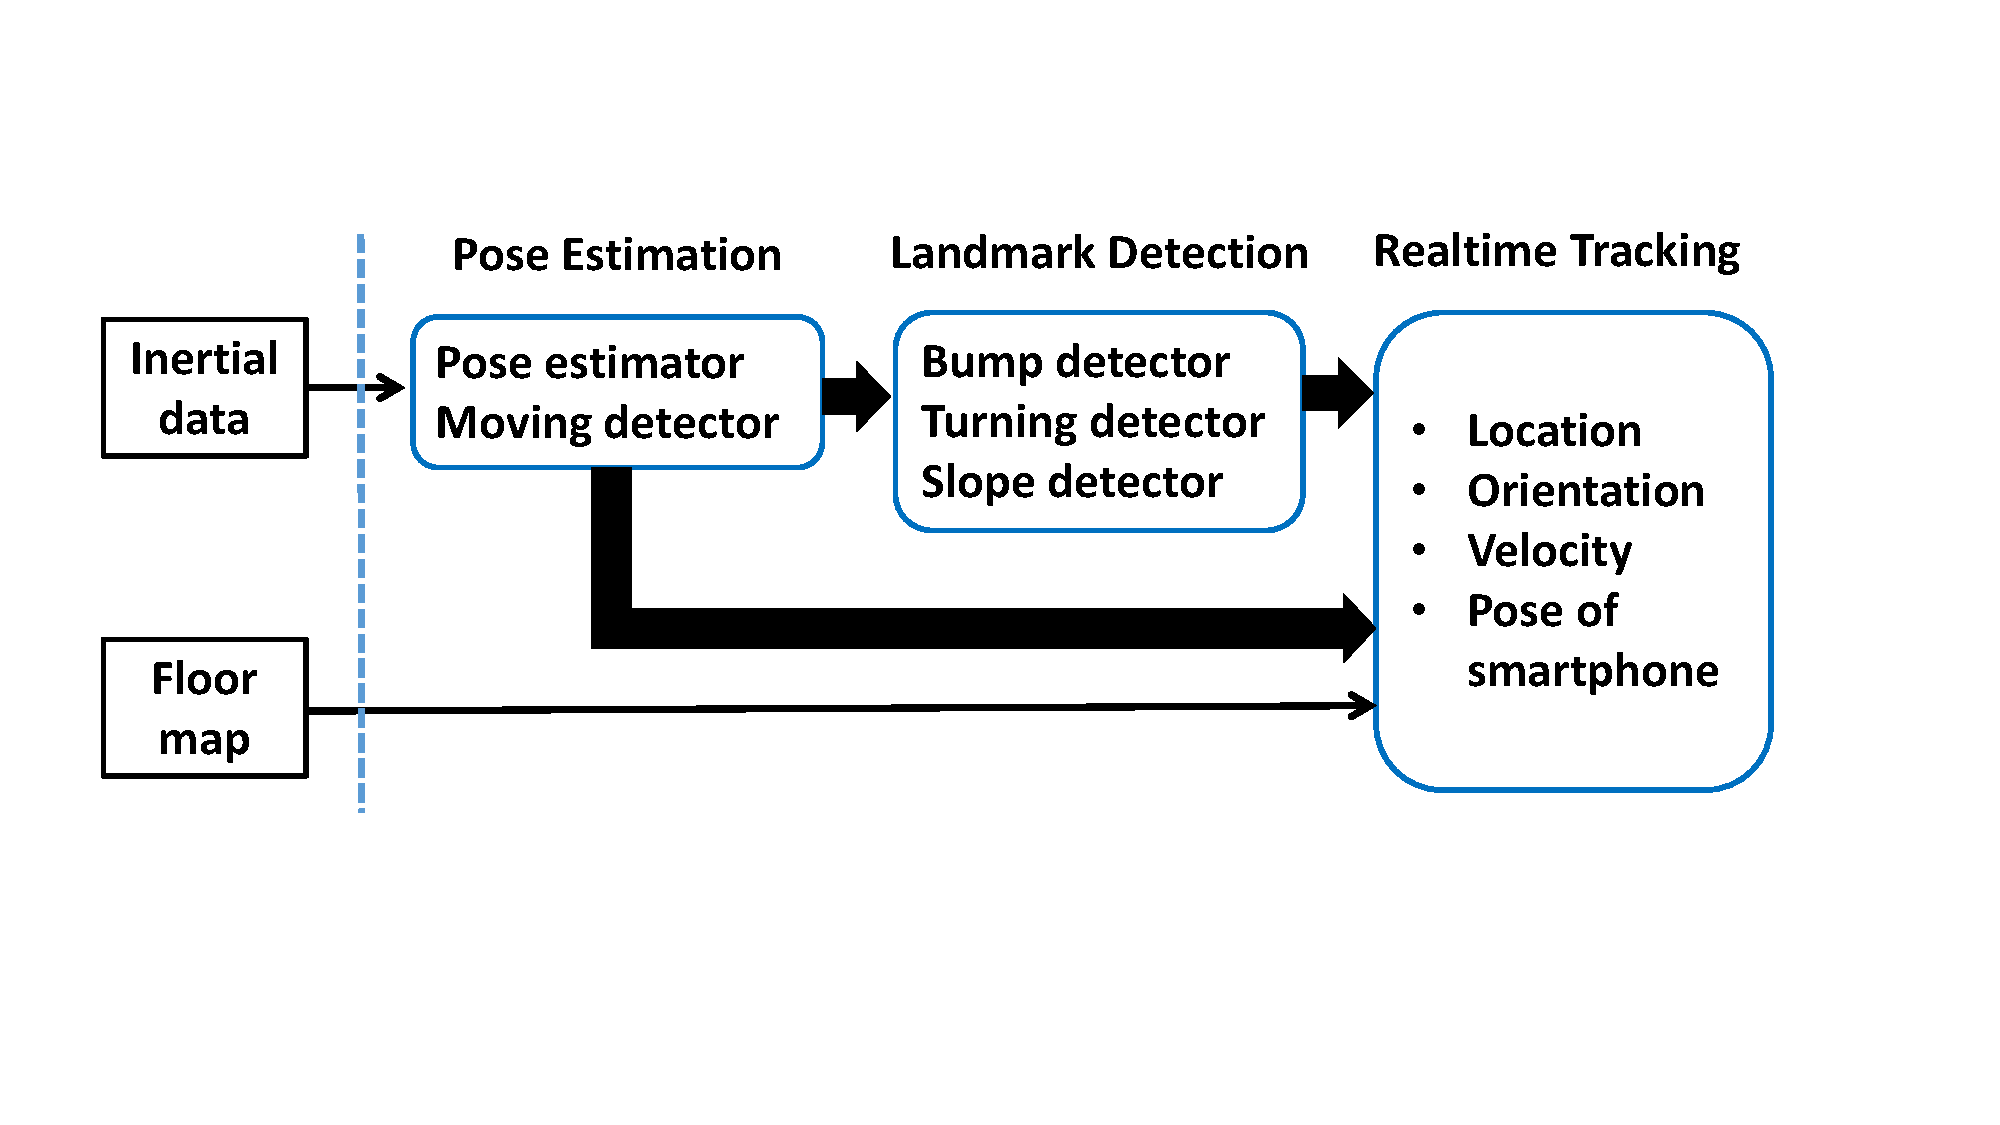
\includegraphics[width=0.5\textwidth]{overview}\\
  \caption{Three components of VeLoc. Inertial data is used to compute the smartphone's pose in the vehicle, then it is further processed to detect certain landmarks during driving, and the augmented particle filter harnesses constraints from landmark detection and the floor map for vehicle localization.}\label{pix:overview}
\end{figure}

\iffalse
Specifically, we make the following contributions in this work:

\iffalse
VeLoc contains several components to deal with the above challenges.
A \textit{pose estimation} module estimates the pose of the smartphone inside the vehicle, regardless of how the phone is oriented relative to the vehicle and occasional changes in its pose due to bumpy driving. We also develop a \textit{landmark detection} module which uses pattern recognition and machine learning techniques~\cite{} to find unique patterns corresponding to different types of landmarks and implement real-time classification algorithm to detect them reliably.
Finally, we design a novel Bayes Filtering framework, specifically, \textit{Augmented Particle Filtering} framework using probability distributions to represent the uncertainty about the state of the vehicle, which can be diminished by constraints imposed by the map and detected landmarks.
\fi

%Finally, we represent the uncertainty about the state of the vehicle explicitly as probability distributions. We incorporate the uncertainty arising from sensing and the parking structure's map information provided by the map or detected landmarks, into a novel Bayes Filtering framework, specifically, \textit{ Augmented Particle Filtering} framework to simultaneously harness constraints imposed by the map and landmark detection for localization. (xx last sentence still too long and vague. need to sharpen the point)


%(Contribution)

\begin{itemize}
  \item We develop a robust pose estimation algorithm that can handle arbitrary orientations of the phone in the vehicle and possible jolting that alters the pose during the course of driving. We identify a set of landmarks commonly encountered in parking structures, and propose respective detection algorithms to classify them reliably.
  \item We identify an opportunity to simultaneously harness constraints imposed by the parking structure's map and detected landmarks for localization. We formulate such constraints into a Bayes Filtering framework that uses probability distributions to represent the vehicle state, and infers the final location by reducing the uncertainty using the map and detected landmarks.
  \item We implement a prototype and conduct extensive experiments using different parking structures, vehicles and driving styles to evaluate the robustness and accuracy of VeLoc. We find that it can locate the vehicle within $10m$, which is sufficient for the remote key to trigger a honking sound. The pose can be estimated with 9 degrees error, which is fast enough to deal with occasional jolting in real time. % We also implement the algorithms in a smartphone app that can run in real time to track the vehicle's location, which demonstrate the computation efficiency of our design.
\end{itemize}

The rest of this paper is organized as follows: we give a brief design overview in Section~\ref{sec:overview}. We then propose a pose estimation algorithm for the smartphone inside a vehicle in Section~\ref{sec:pose}, and landmark detection algorithms in Section~\ref{sec:landmark}. Additionally, Section~\ref{sec:tracking} presents our sequential importance re-sampling framework. We report experimental evaluation in Section~\ref{sec:evaluation}, and review the related work in Section~\ref{sec:background}. After a discussion of limitations in Section~\ref{sec:discussion}, we conclude the paper in Section~\ref{sec:conclusion}.
\fi


The intuition behind VeLoc is that although a noisy trajectory does not, by itself, reveal a vehicle's location, using the constraints imposed by the parking structure��s map and detected landmarks is able to help vehicle tracking(shown in Figure \ref{fig_poster}).
%This is because (a) trajectories can be used for localization since only a few paths on the map could accommodate the trajectory. (b) once a landmark is detected, only a few positions marked with the same kind of landmark are possible. (c) using both map constraints and detected landmark could narrow down the uncertainty more quickly and trace a vehicle more accurately. 

\begin{figure}[h]
      \centering
      \vspace{-10pt}
        \subfigure[Localization using constraints imposed by the map.] {
        \begin{minipage}[b]{0.5\textwidth}
        \centering
        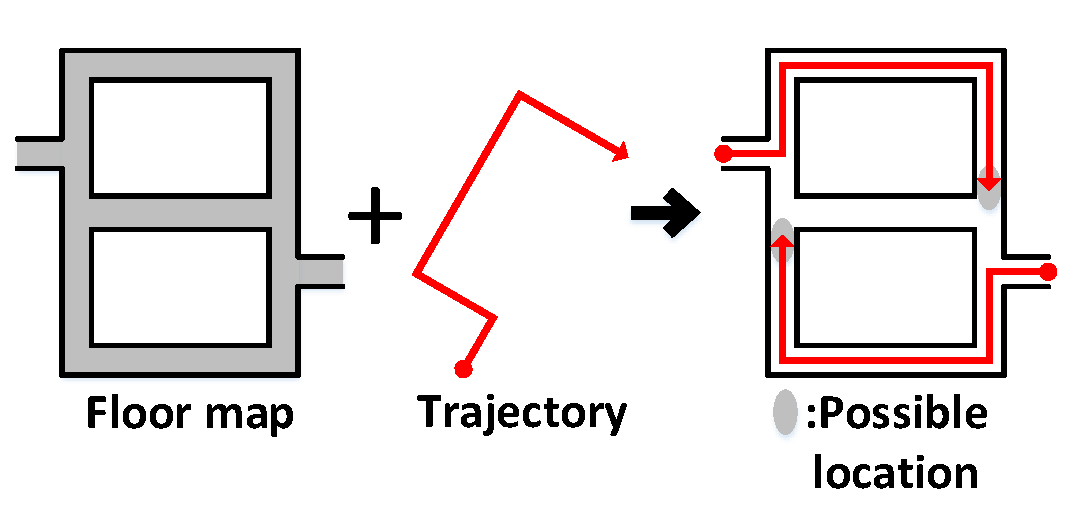
\includegraphics[width=0.8\textwidth]{apf1}\label{fig_apf_intuition1}
        \end{minipage}
        }
        \subfigure[Localization using detected landmarks.] {
        \begin{minipage}[b]{0.5\textwidth}
        \centering
        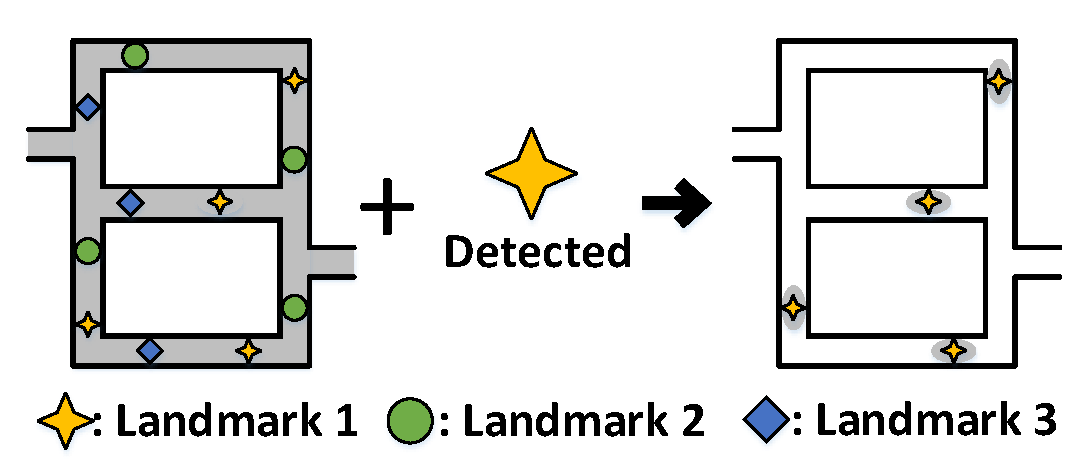
\includegraphics[width=0.8\textwidth]{apf2}\label{fig_apf_intuition2}
        \end{minipage}
        }
        \subfigure[Localization using both map constraints and detected landmarks.] {
        \begin{minipage}[b]{0.5\textwidth}
        \centering
        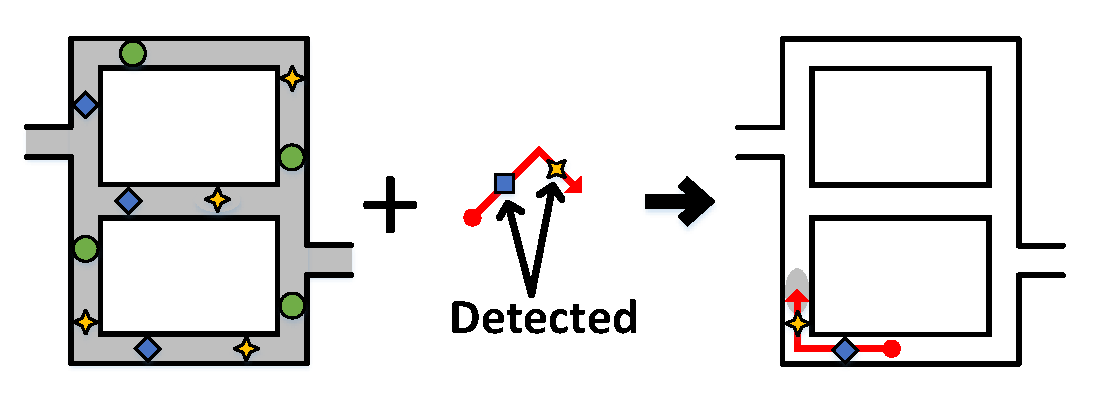
\includegraphics[width=0.8\textwidth]{apf3}\label{fig_apf_intuition3}
        \end{minipage}
        }
        \vspace{-4pt}
        \caption{Intuition of localization.
        (a) trajectories can be used for localization since only a few paths on the map could accommodate the trajectory. (b) once a landmark is detected, only a few positions marked with the same kind of landmark are possible. (c) using both map constraints and detected landmark could narrow down the uncertainty more quickly.}
        \label{fig_poster}
\end{figure}